\documentclass[10pt,english]{scrartcl}
\usepackage{babel}
\usepackage{shortvrb}
\usepackage[latin1]{inputenc}
\usepackage{tabularx}
\usepackage{longtable}
\setlength{\extrarowheight}{2pt}
\usepackage{amsmath}
\usepackage{graphicx}
\usepackage{color}
\usepackage{multirow}
\usepackage[colorlinks=true,linkcolor=blue,urlcolor=blue]{hyperref}
\usepackage[a4paper,margin=2cm,nohead]{geometry}
%% generator Docutils: http://docutils.sourceforge.net/
\newlength{\admonitionwidth}
\setlength{\admonitionwidth}{0.9\textwidth}
\newlength{\docinfowidth}
\setlength{\docinfowidth}{0.9\textwidth}
\newcommand{\optionlistlabel}[1]{\bf #1 \hfill}
\newenvironment{optionlist}[1]
{\begin{list}{}
  {\setlength{\labelwidth}{#1}
   \setlength{\rightmargin}{1cm}
   \setlength{\leftmargin}{\rightmargin}
   \addtolength{\leftmargin}{\labelwidth}
   \addtolength{\leftmargin}{\labelsep}
   \renewcommand{\makelabel}{\optionlistlabel}}
}{\end{list}}
% begin: floats for footnotes tweaking.
\setlength{\floatsep}{0.5em}
\setlength{\textfloatsep}{\fill}
\addtolength{\textfloatsep}{3em}
\renewcommand{\textfraction}{0.5}
\renewcommand{\topfraction}{0.5}
\renewcommand{\bottomfraction}{0.5}
\setcounter{totalnumber}{50}
\setcounter{topnumber}{50}
\setcounter{bottomnumber}{50}
% end floats for footnotes
% some commands, that could be overwritten in the style file.
\newcommand{\rubric}[1]{\subsection*{~\hfill {\it #1} \hfill ~}}
% end of "some commands"
\title{RRADical Pd}
\author{}
\date{}
\hypersetup{
pdftitle={RRADical Pd},
pdfauthor={Frank Barknecht {$<$}fbar@footils.org{$>$}}
}
\raggedbottom
\begin{document}
\maketitle

%___________________________________________________________________________
\begin{center}
\begin{tabularx}{\docinfowidth}{lX}
\textbf{Author}: &
	Frank Barknecht {$<$}fbar@footils.org{$>$} \\
\end{tabularx}
\end{center}
\subsection*{~\hfill Abstract\hfill ~}

The goal of RRADical Pd is to create a collection of patches, that make
Pd easier and faster to use for people who are more used to commercial
software like Reason(tm) or Reaktor(tm).  RRAD as an acronym stands for
``Reusable and Rapid Audio Development'' or ``Reusable and Rapid
Application Development'', if it includes non-audio patches, with Pd. It
is spelled RRAD, but pronounced Rradical. ;)



%___________________________________________________________________________

\hypertarget{what-it-takes-to-be-a-rradical}{}
\section*{What it takes to be a RRADical}
\pdfbookmark[0]{What it takes to be a RRADical}{what-it-takes-to-be-a-rradical}

RRAD as an acronym stands for ``Reusable and Rapid Audio Development'' or
``Reusable and Rapid Application Development'', if it includes non-audio
patches, with Pd. It is spelled RRAD, but pronounced Rradical. ;)

The goal of RRADical Pd is to create a collection of patches, that make Pd
easier and faster to use for people who are more used to software like Reason(tm)
or Reaktor(tm). For that I would like to create patches, that solve real-world
problems on a higher level of abstraction than the standard Pd objects do. 
Where suitable these high level abstractions should have a GUIs
built in.

So for example instead of a basic \texttt{lop{\~{ }}} low pass filter something more
complete like a recreation of the Sherman filter bank could be included in
that collection. My older sseq and angriff patches followed this idea in
general, but there are much more patches needed. Like this:
\begin{itemize}
\item 
a sample player (adapt Gyre?)

\item 
Various OSC/LFO with preset waveforms

\item 
drum machine

\item 
guitar simulator

\item 
grain sample player

\item 
more sequencers

\item 
basically a lot of things like these things in Reason

\end{itemize}

Not that I want to make Pd be Reason, no way. But pre-fabricated high-level
abstractions may not only make Pd easier to use for beginners, they also
can spare lot of tedious, repeating patching work.


%___________________________________________________________________________

\hypertarget{problems-and-solutions}{}
\section*{Problems and Solutions}
\pdfbookmark[0]{Problems and Solutions}{problems-and-solutions}

To building above system several problems are to be solved. Two key areas
already targetted are:
\begin{description}
%[visit_definition_list_item]
\item[\textbf{Persistence}]
%[visit_definition]

How to save the current state of a patch? How to save more than one
state (state sequencing)?

%[depart_definition]
%[depart_definition_list_item]
%[visit_definition_list_item]
\item[\textbf{Communication}]
%[visit_definition]

The various modules are building blocks for a larger application. How
should they talk to each other. (In Reason this is done by patching the
back or modules with horrible looking cables. We must do better.)

%[depart_definition]
%[depart_definition_list_item]
\end{description}

It turned out, that both tasks are possible to solve in a consistent way
using a unique abstraction. But first lets look a bit deeper at the
problems at hand.


%___________________________________________________________________________

\hypertarget{persistence}{}
\subsection*{Persistence}
\pdfbookmark[1]{Persistence}{persistence}

Pd offers no direct way to store the current state of a patch. Here's what
Pd author Miller S. Puckette writes about this in the Pd manual in section
``2.6.2.  persistence of data'':
\begin{quote}

Among the design principles of Pd is that patches should be printable,
in the sense that the appearance of a patch should fully determine its
functionality. For this reason, if messages received by an object
change its action, since the changes aren't reflected in the object's
appearance, they are not saved as part of the file which specifies the
patch and will be forgotten when the patch is reloaded.
\end{quote}

(I'll show an example of a float object changing ``state'' by a message in
its right inlet here.)

Still, in a musician's practice some kind of persistence turns out to be an
important feature, that many Pd beginners do miss. So there are several
approaches to add it. Max/MSP has the \texttt{preset}-object, Pd has the
\texttt{state}-object which saves the current state of (some) GUI objects inside
a patch. Both also support changing between several different states.

Both have at least two problems: They save only the state of GUI objects,
which might not be all that a user wants to save. And they don't handle
abstractions very well, which are crucial when creating modularized
patches.

Another approach is to (ab)use some of the Pd objects that can persist
itself to a file, especially \texttt{textfile}, \texttt{qlist} and \texttt{table}, which
works better, but isn't standardized.

A rather new candidate for state saving is Thomas Grill's \texttt{pool}
external. Basically it offers something, that is standard in many
programming languages: a data structure that stores key-value-pairs. This
also is known as hash, dictonary or map. With \texttt{pool} those pairs also can
be stored in hierarchies and they can be saved to or loaded from disk. The
last but maybe most important feature for us is, that several pools can be
shared by giving them the same name. A \texttt{pool MYPOOL} in one patch will
contain the same data as a \texttt{pool MYPOOL} in another patch. Changes to one
pool will change the data in the other as well.

A \texttt{pool} object is central to the persistence in RRADical patches, but it
is hidden behind an abstracted ``API'', if one could name it that. I'll
come back to haw this is done late.


%___________________________________________________________________________

\hypertarget{communication}{}
\subsection*{Communication}
\pdfbookmark[1]{Communication}{communication}

Besides persistance it also is important to create a common path through
which the RRADical modules will talk to each other. Generally the modules
will have to use, what Pd offers them, and that is either a direct
connection through patch cords or the indirect use of the send/receive
mechanism in Pd. Patch cords are fine, but tend to clutter the interface.
Sends and receives on the other hand will have to make sure, that no name
clashes occur. A name clash is, when one target receives messages not
intended for it. A patch author has to remember all used send-names, but
this gets harder, if he uses prefabricated modules, which might use their
own senders.

So it is crucial, that senders in RRADical abstractions use local senders
only with as few exceptions as possible. This is achieved by prepending the
RRADical senders with the string ``{\$}0-''. So you'd not use \texttt{send volume},
but instead use \texttt{send {\$}0-volume}. {\$}0 makes those sends local inside their
own patch borders. This might be a bit difficult to understand to the
casual Pd user, but is a pretty standard idiom in the Pd world.

Still we will want to control a lot of parameters and do so not only
through the GUI Pd offers, but probably also through other ways, for
example through Midi controllers, through some kind of score on disk,
through satellite navigation receivers or whatever.

This creates a fundamental conflict:
\begin{description}
%[visit_definition_list_item]
\item[\textbf{We want borders}   ]
%[visit_definition]

We want to separate our abstraction so they don't conflict with each
other.

%[depart_definition]
%[depart_definition_list_item]
%[visit_definition_list_item]
\item[\textbf{We want border crossings}]
%[visit_definition]

We want to have a way to reach their many internals and control them
from the outside.

%[depart_definition]
%[depart_definition_list_item]
\end{description}

The RRADical approach adheres to this in that it enforces a strict border
but drills a single hole in it: the \textbf{OSC inlet}. This idea is the result
of a discussion on the Pd mailing list and goes back to suggestions by
\href{http://www.audionerd.com}{Eric Skogen} and \href{http://www.ekran.org/ben/}{Ben Bogart}. Every RRADical patch has (to have) a
rightmost inlet that accepts messages formatted according to the OSC
protocol. OSC stands for \href{http://www.cnmat.berkeley.edu/OpenSoundControl/}{Open Sound Control} and is a network transparent
system to control audio applications remotely developed at CNMAT in Berkley.

The nice thing about OSC is that it can control many parameters over a
single communication path. This is so, because OSC uses a URL-like scheme
to address parameters. An example would be this message:
\begin{ttfamily}\begin{flushleft}
\mbox{/synth/fm/volume~85}
\end{flushleft}\end{ttfamily}

It sends the message ``85'' to the ``volume'' control of a ``fm'' module below a
``synth'' module. OSC allows many parameters constructs like:
\begin{ttfamily}\begin{flushleft}
\mbox{/synth/fm/basenote~~~~~~~~~~~~~~52}\\
\mbox{/synth/virtualanalog/basenote~~~40}\\
\mbox{/synth/*/playchords~~~~~~~~~~~~~m7b5~M6~7b9}
\end{flushleft}\end{ttfamily}

This might set the base note of two synths, fm and virtualanalog and
send a chord progression to be played by both -- indicated by the wildcard
* -- afterwards.

The OSC-inlet of every RRADical patch is intended as the border crossing:
Everything the author of a certain patch intends to be controlled from the
outside can be controlled by OSC messages to the rightmost inlet.


%___________________________________________________________________________

\hypertarget{trying-to-remember-it-all-memento}{}
\section*{Trying to remember it all: Memento}
\pdfbookmark[0]{Trying to remember it all: Memento}{trying-to-remember-it-all-memento}

To realize the functionality requirements developed so far I resorted to a
so called Memento. ``Memento'' is a very cool movie by director
Christopher Nolan where - quoting IMDB:
\begin{quote}

A man, suffering from short-term memory loss, uses notes and tattoos to
hunt down his wife's killer.
\end{quote}

If you haven't already done so: Watch this movie! It's much better than
Matrix 2 and 3 and also stars Carrie-Anne ``Trinity'' Moss.

Here's a scene from ``Memento'':

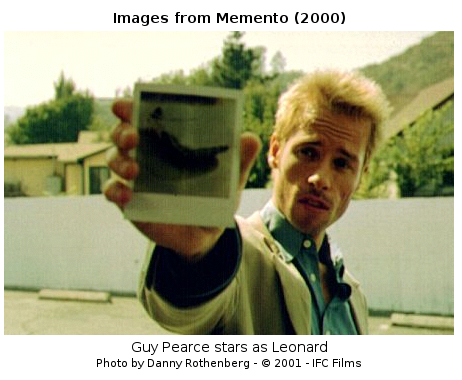
\includegraphics{memento.png}

We see the film's main character Leonard who has a similar problem as Pd: he
cannot remember things. To deal with his persistence problem, his inability
to save data to his internal harddisk he resorts to taking a lot of photos.
These pictures act as what is called a Memento: a recording of the current
state of things.

In software development Mementos are quite common as well. The computer
science literature describes them in great detail. To make the best use of
a Memento science recommends an approach where certain tasks are in the
responsibility of certain independent players.

The Memento itself, as we have seen, is the photo, i.e. some kind of state
record. A module called the ``Originator'' is responsible for creating this
state and managing changes in it.  In the movie, Leonard is the Originator,
he is the one taking photos of the world he is soon to forget.

The actual persistence, that could be the saving of a state to harddisk,
but could just as well be an upload to a webserver or a CVS check-in, is
done by someone called the ``Caretaker'' in the literature. A Caretaker could
be a safe, where Leonard puts his photos, or could be a person, to whom
Leonard gives his photos. In the movie Leonard also makes ``hard saves'' by
tattooing himself with notes he took. In that case, he is not only the
Originator of the notes, but also the Caretaker in one single person.  The
Caretaker only has to take care, that those photos, the Mementos, are in a
safe place and noone fiddles around with them. Btw: In the movie some
interesting problems with Caretakers, who don't always act responsible,
occur.


%___________________________________________________________________________

\hypertarget{memento-in-pd}{}
\subsection*{Memento in Pd}
\pdfbookmark[1]{Memento in Pd}{memento-in-pd}

I developed a set of abstractions, of patches for Pd, that follow this
design pattern. Memento for Pd includes a \texttt{caretaker} and an
\texttt{originator} abstraction, plus a third one called \texttt{commun} which is
responsible for the \textbf{internal} communication. \texttt{commun} basically is
just a thin extension of \texttt{originator} and should be considered part of
it.  There is another patch, the \texttt{careGUI} which I personally use instead
of the \texttt{caretaker} directly, because it has a simple GUI included.

Here's how it looks:

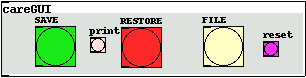
\includegraphics{caregui.png}

The \texttt{careGUI} is very simple: select a FILE-name to save to, then
clicking SAVE you can save the current state, with RESTORE you can restore
a state previously saved. After restore, the outlet of \texttt{careGUI} sends a
\texttt{bang} message to be used as you like.

Internally \texttt{caretaker} has a named \texttt{pool} object using the global pool
called ``RRADICAL''. The same \texttt{pool RRADICAL} also is used inside the
\texttt{originator} object. This abstraction handles all access to this pool. A
user should not read or write the contents of \texttt{pool RRADICAL} directly.
The \texttt{originator} patch also handles the border crossing through OSC
messages by it's rightmost inlet. The patch accepts two mandatory
arguments: The first on is the name under which this patch is to be stored
inside the \texttt{pool} data. Each \texttt{originator SomeName secondarg}  stores
it's data in a virtual subdirectory inside the RRADICAL-pool called like
its first argument - SomeName in the example. If the SomeName starts with a
slash like ``/patch'' , you can also accesse it via OSC through the rightmost inlet of
\texttt{originator} under the tree ``/patch''

The second argument practically always will be {\$}0. It is used to talk to
those \texttt{commun} objects which share the same second argument. As {\$}0 is a
value local and unique to a patch (or to an abstraction to be correct) each
\texttt{originator} then only can talk to \texttt{commun}s inside the same patch and
will not disturb other \texttt{commun} objects in other abstractions.

The \texttt{commun} objects finally are where the contents of a state are read
and set. They, too, accept two arguments, the second of which was
discussed before and will most of the time just be {\$}0. The first argument
will be the key under which some value will be saved. You should use a slash
as first character here as well to allow OSC control. So an example for a
usage would be \texttt{commun /vol {\$}0}.

\texttt{commun} has one inlet and one outlet. What comes in through the inlet is
send to \texttt{originator} who stores it inside its Memento under the key, that
is specified by the \texttt{commun}'s first arg. Actually \texttt{originator}. The
outlet of a \texttt{commun} will spit out the current value stored under its key
inside the Memento, when \texttt{originator} tells it to do so. So \texttt{commun}s
are intended to be cross-connected to some thing that can change. And
example would be a slider which can be connected as seen in the next
picture:

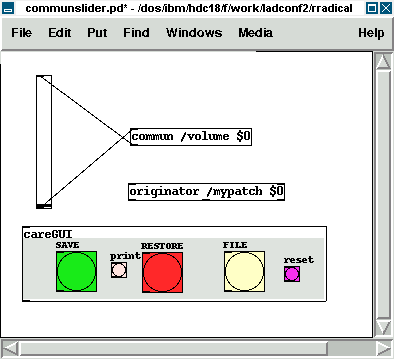
\includegraphics{communslider.png}

In this patch, every change to the slider will be reflected inside the
Memento. The little print button in \texttt{careGUI} can be used to print the
contents to the console from which Pd was started. Setting the slider will
result in something like this:
\begin{ttfamily}\begin{flushleft}
\mbox{/mypatch~0~,~/volume~,~38}
\end{flushleft}\end{ttfamily}

Here a comma separates key and value pairs. ``mypatch'' is the toplevel
directory. This contains a 0, which is the default subdirectory, after that
comes the key ``/volume'', whose value is 38. Let's add another slider for
pan-values:

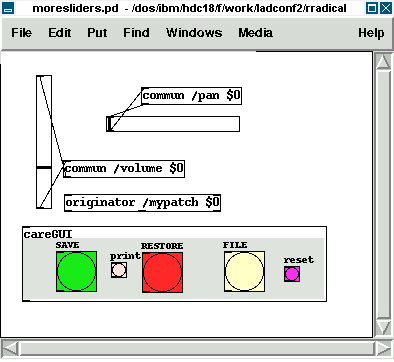
\includegraphics{moresliders.png}

Moving the /pan slider will let careGUI print out:
\begin{ttfamily}\begin{flushleft}
\mbox{/mypatch~0~,~/volume~,~38}\\
\mbox{/mypatch~0~,~/pan~,~92}
\end{flushleft}\end{ttfamily}

The \texttt{originator} can save several substates or presets by sending a
\texttt{substate {\#}number} message to its first inlet. Let's do just this and
move the sliders again as seen in the next picture:

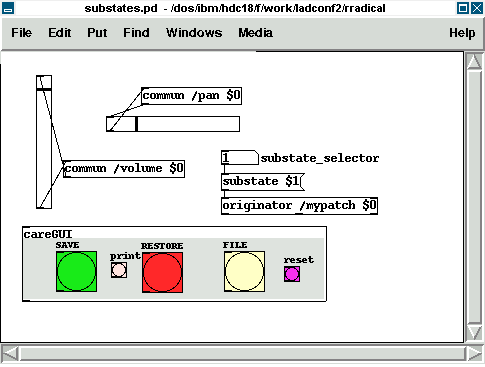
\includegraphics{substates.png}

Now careGUI prints:
\begin{ttfamily}\begin{flushleft}
\mbox{/mypatch~0~,~/volume~,~38}\\
\mbox{/mypatch~0~,~/pan~,~92}\\
\mbox{/mypatch~1~,~/volume~,~116}\\
\mbox{/mypatch~1~,~/pan~,~27}
\end{flushleft}\end{ttfamily}

You see, the substate 0 is unaffected, the new state can have different
values. Exchanging the \texttt{substate} message with a \texttt{setsub} message will
autoload the selected state and ``set'' the sliders to the stored values
immediatly.


%___________________________________________________________________________

\hypertarget{osc-in-memento}{}
\subsection*{OSC in Memento}
\pdfbookmark[1]{OSC in Memento}{osc-in-memento}

The whole system now already is prepared to be used over OSC. You probably
already guess, how the message looks like. Any takers? Thank you, you're
right, the messages are built as \texttt{/mypatch/volume {\#}number} and
\texttt{/mypatch/pan {\#}number} as shown in the next stage:

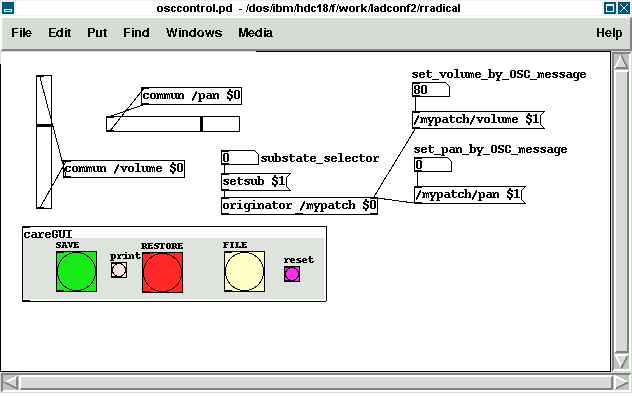
\includegraphics{osccontrol.png}

Sometimes it is useful to also get OSC messages out of a patch, for example
to control other OSC software through Pd. For this the \textbf{OSC-outlet} of
\texttt{originator} can be used, which is the rightmost outlet of the
abstraction. It will print out every change to the current state.
Connecting a \texttt{print OSC} debug object to it, we get to see what's coming
out of the OSC-outlet when we move a slider:
\begin{ttfamily}\begin{flushleft}
\mbox{OSC:~/mypatch/pan~92}\\
\mbox{OSC:~/mypatch/pan~91}\\
\mbox{OSC:~/mypatch/pan~90}\\
\mbox{OSC:~/mypatch/pan~89}
\end{flushleft}\end{ttfamily}


%___________________________________________________________________________

\hypertarget{putting-it-all-to-rradical-use}{}
\section*{Putting it all to RRADical use}
\pdfbookmark[0]{Putting it all to RRADical use}{putting-it-all-to-rradical-use}

Now that the foundation for a general preset and communication system are
set, it is possible to build real patches with it that have two main
characteristics:
\begin{description}
%[visit_definition_list_item]
\item[\textbf{Rapidity}]
%[visit_definition]

Ready-to-use highlevel abstraction can save a lot of time when building
larger patches. Clear communication paths will let you think faster and
more about the really important things.

%[depart_definition]
%[depart_definition_list_item]
%[visit_definition_list_item]
\item[\textbf{Reusability}]
%[visit_definition]

Don't reinvent the wheel all the time. Reuse patches like instruments
for more than one piece by just exchanging the Caretaker-file used.

%[depart_definition]
%[depart_definition_list_item]
\end{description}

I already developed a growing number of patches that follow the RRADical
paradigm, among these are a complex pattern sequencer, some synths and
effects and more. The RRADical collection comes with a template file,
called \texttt{rrad.tpl} that makes deploying new RRADical patches easier and
lets developers concentrate on the algorighm instead of bookeeping. Some
utils (footils?) help with creating the sometimes needed many
\texttt{commun}-objects. Several usecases show example applications of the
provided abstractions.

\end{document}
